%%%%%%%%%%%%%%%%%%%%%%%%%%%%%%%%%%%%%%%%%%%%%%%%%%%%%%%%%%%%%%%%%%%%%%%%%%%

\documentclass[a4paper,oneside,12pt]{article}
\usepackage{mystyle}

\begin{document}

\title{\Large\bf Factoring a quadratic function}
\author{%%
  Minh Van Nguyen \\
  \url{mvngu@gmx.com}
}
\date{\today}
\maketitle


%%%%%%%%%%%%%%%%%%%%%%%%%%%%%%%%%%%%%%%%%%%%%%%%%%%%%%%%%%%%%%%%%%%%%%%%%%%

\section{Factoring}

This document will show you how to factorise a quadratic function.
One reason why you would factorise a quadratic function is so that you
can determine the roots of the function without using the quadratic
formula.  To factorise an expression means to write the expression as
the product of two or more expressions.  In the case of the number
$6$, you can factorise $6$ by writing it as the product of $2$ and
$3$.  Hence the integer $6$ can be written in factored form as
\[
6
=
2 \times 3
\]
and you say that $2$ and $3$ are factors of $6$.  As another example,
you can write $60$ in factored form as $60 = 3 \times 20$.  You can
also factorise $20$ to get $20 = 4 \times 5$ and therefore $60$ can be
factorised as
\[
60
=
3 \times 4 \times 5.
\]
As can be seen from the above examples, factorising an integer
involves writing the integer as the product of two or more integers.
The factors are usually prime integers.  A factorisation of the form
$5 = 1 \times 5$ is correct because $5$ is a prime and has no factors
other than $1$ and $5$.  The factored form $5 = 1 \times 5 \times 1$
is also correct, but that's cheating.

What about factoring quadratic functions?  Let's start with quadratic
functions of the form $f(x) = ax^2 + bx$, where $a$ and $b$ are any
real numbers such that $a \neq 0$.  Use the distributive laws to write
$f(x)$ in the factorised form
%%
\begin{equation}
\label{eqn:factorise_axx_bx}
f(x)
=
(ax + b)x
\end{equation}
%%
to see that $f(x)$ has the factors $x$ and $ax + b$.  Looking at the
factored form~\eqref{eqn:factorise_axx_bx}, the roots of $f(x)$ are
$x = 0$ and $x = -b/a$.  But how did you get those numbers?  To
calculate the roots of $f(x)$ means to determine all values of $x$
such that the expression $f(x) = 0$ is true.  In other words, you want
to determine all values of $x$ such that the expression
%%
\begin{equation}
\label{eqn:roots_of_axx_bx}
(ax + b)x
=
0
\end{equation}
%%
is true.  Expression~\eqref{eqn:roots_of_axx_bx} tells you that there
are two numbers, i.e.~$x$ and $ax + b$, whose product is zero.  You
have two cases:
%%
\begin{packedenumeral}
\item If $x = 0$, then \Expression{eqn:roots_of_axx_bx} is true
  because zero multiplied by another number is zero.  So one root of
  $f(x)$ is $x = 0$.

\item If $ax + b = 0$, then \Expression{eqn:roots_of_axx_bx} is also
  true.  But for which values of $x$ would you have $ax + b = 0$?
  Solving the latter expression for $x$ shows that $x = -b / a$.
  Substitute the last expresssion into~\eqref{eqn:roots_of_axx_bx}
  produces
  %%
  \begin{align*}
  \squarebracket*{
    a \parenthesis*{-\frac{b}{a}}
    +
    b
  }
  \parenthesis*{-\frac{b}{a}}
  &=
  (-b + b)
  \parenthesis*{-\frac{b}{a}} \\[4pt]
  &=
  0 \times \parenthesis*{-\frac{b}{a}} \\[4pt]
  &=
  0
  \end{align*}
  %%
  which is true.  Hence you have found that $x = -b / a$ is another
  root of $f(x)$.
\end{packedenumeral}
%%
By writing $f(x)$ as the factored form~\eqref{eqn:factorise_axx_bx}
you can easily determine the roots of $f(x)$ without using the
quadratic formula.  The above discussion is summarised in the
following theorem.

\begin{theorem}
\label{thm:quadratic_function_vertical_intercept_zero}
Consider the quadratic function $f(x) = ax^2 + bx$, where $a$ and $b$
are any real numbers such that $a \neq 0$.  The roots of $f(x)$ are
\[
x = 0
%%
\qquad
\text{and}
\qquad
%%
x = -\frac{b}{a}.
\]
\end{theorem}

\begin{example}
\label{eg:AmazingCar}
\textbf{AmazingCar.}
At a particular toy store, the sales of a toy called AmazingCar is
given by the sales function $S(x) = -3x + 40$.  Here $x$ represents
the price in dollars of each unit of AmazingCar and so $x$ is the unit
price.  The sales function $S(x)$ represents the number of units of
AmazingCar sold during a week.
%%
\begin{packedenum}
\item\label{subeg:AmazingCar_graph_sales_function}
  Produce a graph of the sales function.  Use the graph to help you
  explain the sales function.  Identify the unit prices at which the
  number of units of AmazingCar sold is highest and lowest.

\item\label{subeg:AmazingCar_revenue_function}
  Derive an expression for the revenue from selling units of
  AmazingCar during a particular week.  Produce a graph of the revenue
  function.

\item\label{subeg:AmazingCar_price_zero_revenue}
  At which unit prices would the revenue from selling units of
  AmazingCar be zero dollars during a week?
\end{packedenum}
\end{example}

\begin{solution}
\solutionpart{subeg:AmazingCar_graph_sales_function}
\Figure{fig:AmazingCar_sales} shows a graph of the sales function
$S(x)$.  The graph shows that as the price for each unit of AmazingCar
increases the lower is the number of units sold during a week.  In
other words, the lower is the unit price the higher is the number of
units sold during the week.  This sounds reasonable because as the
price of something decreases you would expect to sell more of the
product.  Note the two points on the graph that show the lowest and
highest number of units sold.  These are the intercepts of the axes.
The horizontal intercept is the point $\tuple{\frac{40}{3}}{0}$, which
tells you that when the unit price is approximately $\$13.33$ zero
units of AmazingCar would be sold per week.  The lowest number of
units sold per week is zero.  The vertical intercept $\tuple{0}{40}$
tells you that when the unit price is zero dollars~(each unit of
AmazingCar is given away free of charge), the number of units sold per
week is $40$, which is also the highest number of units sold per
week.

\begin{figure}[!htbp]
\centering
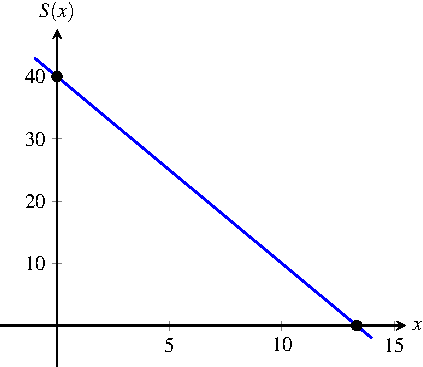
\includegraphics[scale=1.1]{image/10/amazingcar-sales.pdf}
\caption{%%
  Graph of the sales function $S(x) = -3x + 40$ for AmazingCar.  Here
  $x$ represents the unit price in Australian dollars and $S(x)$
  represents the number of units of AmazingCar sold at $x$ dollars
  per unit.
}
\label{fig:AmazingCar_sales}
\end{figure}

\solutionpart{subeg:AmazingCar_revenue_function}
Since $x$ is the unit price and $S(x)$ represents how many units were
sold during a week, the revenue from selling AmazingCar is the
expression
\[
R(x)
=
x S(x)
=
x(-3x + 40).
\]
The revenue function is graphed in \Figure{fig:AmazingCar_revenue}.

\begin{figure}[!htbp]
\centering
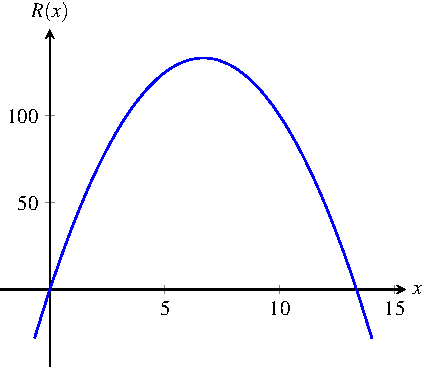
\includegraphics[scale=1.1]{image/10/amazingcar-revenue.pdf}
\caption{%%
  Graph of the revenue function $R(x) = x(-3x + 40)$ for AmazingCar.
  The function $R(x)$ represents the revenue~(in dollars) from selling
  units of AmazingCar during a week at $x$ dollars per unit.
}
\label{fig:AmazingCar_revenue}
\end{figure}

\solutionpart{subeg:AmazingCar_price_zero_revenue}
\Figure{fig:AmazingCar_revenue} shows that you have two unit prices at
which the revenue from selling AmazingCar would be zero dollars during
a week.  Those particular two unit prices are the roots of $R(x)$.
You can use the quadratic formula to determine the roots of $R(x)$.
However, note that you can use the distributive laws to write the
revenue function as
%%
\begin{equation}
\label{eqn:AmazingCar_revenue_function_distributive}
R(x)
=
-3x^2 + 40x.
\end{equation}
%%
You then use \Theorem{thm:quadratic_function_vertical_intercept_zero}
to conclude that the roots of $R(x)$ are $x = 0$ and
\[
x
=
-\frac{40}{-3}
=
\frac{40}{3}.
\]
In other words, the revenue during a week from selling units of
AmazingCar would be zero dollars if the unit prices were either zero
dollars or approximately $\$13.33$.
\end{solution}

\begin{exercise}
\textbf{More AmazingCar.}
You will further explore \Example{eg:AmazingCar}.
%%
\begin{packedenum}
\item\label{subeg:AmazingCar_roots_quadratic_formula}
  Use the quadratic formula to verify the roots of the revenue
  function.

\item\label{subeg:AmazingCar_maximum_revenue}
  Determine the unit price that would result in the maximum revenue
  during a week from selling units of AmazingCar.
\end{packedenum}
\end{exercise}

\ifbool{showSolution}{
\begin{solution}
\solutionpart{subeg:AmazingCar_roots_quadratic_formula}
Apply the quadratic formula on the revenue
function~\eqref{eqn:AmazingCar_revenue_function_distributive} to see
that the roots of $R(x)$ are given by the expression
%%
\begin{align*}
x
&=
\frac{
  -40 \pm \sqrt{40^2 - 4(-3)(0)}
}{
  2(-3)
} \\[4pt]
&=
\frac{
  -40 \pm 40
}{
  -6
}.
\end{align*}
Thus the roots of $R(x)$ are
\[
x
=
\frac{-40 + 40}{-6}
=
0
\]
and
\[
x
=
\frac{-40 - 40}{-6}
=
\frac{40}{3}
\]
which are the same as what you got in \Example{eg:AmazingCar}.

\solutionpart{subeg:AmazingCar_maximum_revenue}
The maximum revenue is located at the vertex in the graph of $R(x)$.
The horizontal coordinate of the vertex is
\[
x
=
\frac{-40}{2(-3)}
=
\frac{20}{3}.
\]
The vertical coordinate of the vertex is
\[
R(20/3)
=
\frac{20}{3}
\parenthesis*{
  -3 \times \frac{20}{3}
  +
  40
}
=
\frac{20}{3}
(-20 + 40)
=
\frac{400}{3}.
\]
That is, the maximum revenue during a week from selling units of
AmazingCar would be approximately $\$133.33$, which would occur if the
unit price is approximately $\$6.67$.  All numbers have been rounded
to two decimal places.
\end{solution}
}{}


%%%%%%%%%%%%%%%%%%%%%%%%%%%%%%%%%%%%%%%%%%%%%%%%%%%%%%%%%%%%%%%%%%%%%%%%%%%

\section{Completing the square}

\begin{figure}[!htbp]
\centering
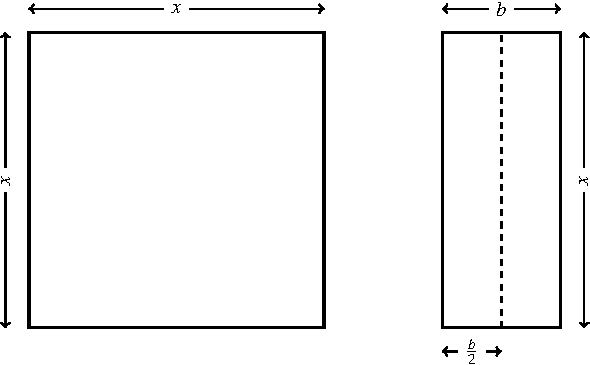
\includegraphics[scale=1.1]{image/10/complete-square-a1-c0.pdf}
\caption{%%
  The quadratic function $f(x) = x^2 + bx$ can be visualised as a
  square plus a rectangle.  The square has a side length of $x$, hence
  the area of the square is $x^2$.  The rectangle has a width of $b$
  and a height of $x$, so the rectangle has an area of $bx$.  Thus
  $f(x)$ can be interpreted as the area of a square plus the area of a
  rectangle.  The rectangle can be cut in half along the dashed line
  as shown.  Each half has a width of $b/2$ and a height of $x$.
}
\label{fig:special_complete_square_square_plus_rectangle}
\end{figure}

\begin{figure}[!htbp]
\centering
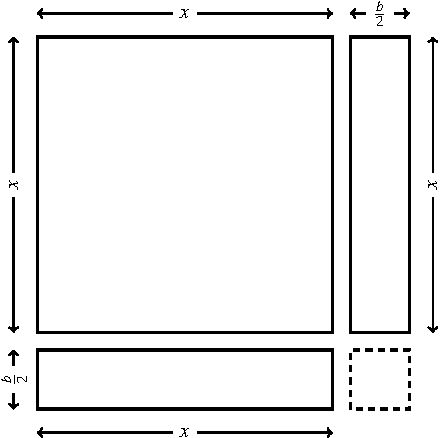
\includegraphics[scale=1.1]{image/10/complete-square-a1-c0_halfb.pdf}
\caption{%%
  The quadratic function $f(x) = x^2 + bx$ can be visualised as a
  square plus a rectangle.  The rectangle is cut in half.  One half is
  arranged to the right of the square.  The other half is arranged
  underneath the square.  Now you have a shape that is nearly like a
  square.  The small dashed square in the lower right is what is
  missing to make a complete square.
}
\label{fig:}
\end{figure}

\end{document}
